% Template for PLoS
% Version 1.0 January 2009
%
% To compile to pdf, run:
% latex plos.template
% bibtex plos.template
% latex plos.template
% latex plos.template
% dvipdf plos.template

\documentclass[10pt]{article}

% amsmath package, useful for mathematical formulas
\usepackage{amsmath}
% amssymb package, useful for mathematical symbols
\usepackage{amssymb}

% graphicx package, useful for including eps and pdf graphics
% include graphics with the command \includegraphics
\usepackage{graphicx}
\usepackage{wrapfig}
\usepackage{floatrow}
\usepackage{subfig}
% cite package, to clean up citations in the main text. Do not remove.
\usepackage{cite}

\usepackage{color} 

% Use doublespacing - comment out for single spacing
%\usepackage{setspace} 
%\doublespacing


% Text layout
\topmargin 0.0cm
\oddsidemargin 0.5cm
\evensidemargin 0.5cm
\textwidth 16cm 
\textheight 21cm

% Bold the 'Figure #' in the caption and separate it with a period
% Captions will be left justified
%\usepackage[labelfont=bf]{caption}
%,labelsep=period,justification=raggedright]{caption}
%\captionsetup[subfigure]{labelfont=bf,textfont=normalfont,singlelinecheck=off,justification=raggedright,position=top}


% Use the PLoS provided bibtex style
\bibliographystyle{plos2009}

% Remove brackets from numbering in List of References
\makeatletter
\renewcommand{\@biblabel}[1]{\quad#1.}
\makeatother


% Leave date blank
\date{}

\pagestyle{myheadings}
%% ** EDIT HERE **


%% ** EDIT HERE **
%% PLEASE INCLUDE ALL MACROS BELOW

%% END MACROS SECTION

\begin{document}

% Title must be 150 characters or less
\begin{flushleft}
{\Large
\textbf{From one to many (and back again): an alternating renewal process describes the dynamics of bistable perceptual grouping}
}
% Insert Author names, affiliations and corresponding author email.
\\
Sara Steele$^{1\ast}$, 
Daniel Tranchina$^{2,3}$, 
John Rinzel$^{1,2}$
\\
\bf{1} Center for Neural Science, New York University, New York, NY, USA
\\
\bf{2} Courant Institute for Mathematical Sciences, New York University, New York, NY, USA
\\
\bf{3} Department of Biology, New York University, New York, NY, USA
\\
$\ast$ E-mail: Corresponding steeles@cns.nyu.edu
\end{flushleft}

% Please keep the abstract between 250 and 300 words
\section*{Abstract}
The buildup over time of split percepts for ambiguous stimuli, especially the buildup of stream segregation, has previously been accounted for by feedforward processing as a consequence of the accumulation of adaptation over time. However, 

% Please keep the Author Summary between 150 and 200 words
% Use first person. PLoS ONE authors please skip this step. 
% Author Summary not valid for PLoS ONE submissions.   
\section*{Author Summary}

\section*{Introduction}
For some stimuli in the auditory and visual modalities with ambiguous grouping cues, the probability of perceptual "splitting" increases with time. One example of this buildup is found in auditory stream segregation. A number of studies using ambiguous ABA_ tone sequences \cite{Noorden1975} have shown that perceptual splitting of sound events with different acoustic features requires time to build up \cite{Bregman1978, Anstis1985}.  A and B refer to tones at different frequencies, and _ represents a silent interval. Depending on the the frequency and presentation rate of the tones, listeners might hear grouped triplet patterns or segregated streams of tones at separate frequencies (Figure \ref{fig:percepts_timecourse}). Starting from the initiation of a presentation \cite{Bregman1978, Anstis1985} or a switch in the focus of attention \cite{Cusack2004}, there can be an initial period of buildup over which the probability of the segregated percept increases. A similar phenomenon has been reported in the visual modality. When viewing ambiguous moving plaids constructed from moving square wave gratings at intermediate speed and angle, observers have reported first experiencing coherenct motion of a unified plaid pattern, even when, in the long term, their perception is biased towards transparent motion of the individual gratings \cite{Rubin2004}. The psychophysical observation of this buildup in probability for split perceptual organization is accompanied by reports of perceptual alternations \cite{Dieke2012,Denham,buildup+alternations, some plaid buildups}. That is, because of the ambiguity of the stimuli, subjects report experiencing sudden switches between one perceptual state and the other \cite{Pressnitzer2006, Hupe2012} over long presentations.

Buildup in the auditory domain has been a subject of great interest because it is thought to be a product of the same mechanisms that enable listeners to group components of an acoustic signal according to the sources that produced them. Many explanations of buildup appeal to proposed mechanisms of auditory perceptual organization. One theoretical explanation for the sequential grouping observed with the ABA_ stimuli is grouping by coactivation (for a review, see \cite{Carlyon2004}). Sound signals that excite the same population of neurons are grouped, whereas those which activate separate populations are perceived as coming from separate sources, that is, split. Some theories \cite{Micheyl2005,Pressnitzer2008,Bee2010} propose that the buildup of stream segregation reflects a decrease over time of coactivation of auditory neurons responding to each of the two tone frequencies as a result of the accumulation of adaptation over seconds, or multi-second habituation. %In general, the idea that buildup reflects a process by which the auditory system accumulates evidence is quite old \cite{Bregman1990}. 
The accumulation-based account of buildup can explain the perceptual switch from the grouped to the split percept; however, it is unable to explain why subjects undergo continued switches between percepts. We show that buildup can be described well by a model that uses the statistics of alternations, but no accumulation. The gradual increase in probability of a split percept over time could reflect the dynamics of an entirely random underlying alternating renewal process with a given initial state. In addition, we explore how different mechanisms of alternation affect the model's behavior with regard to buildup.

%\newpage
\begin{figure}
	\centering
	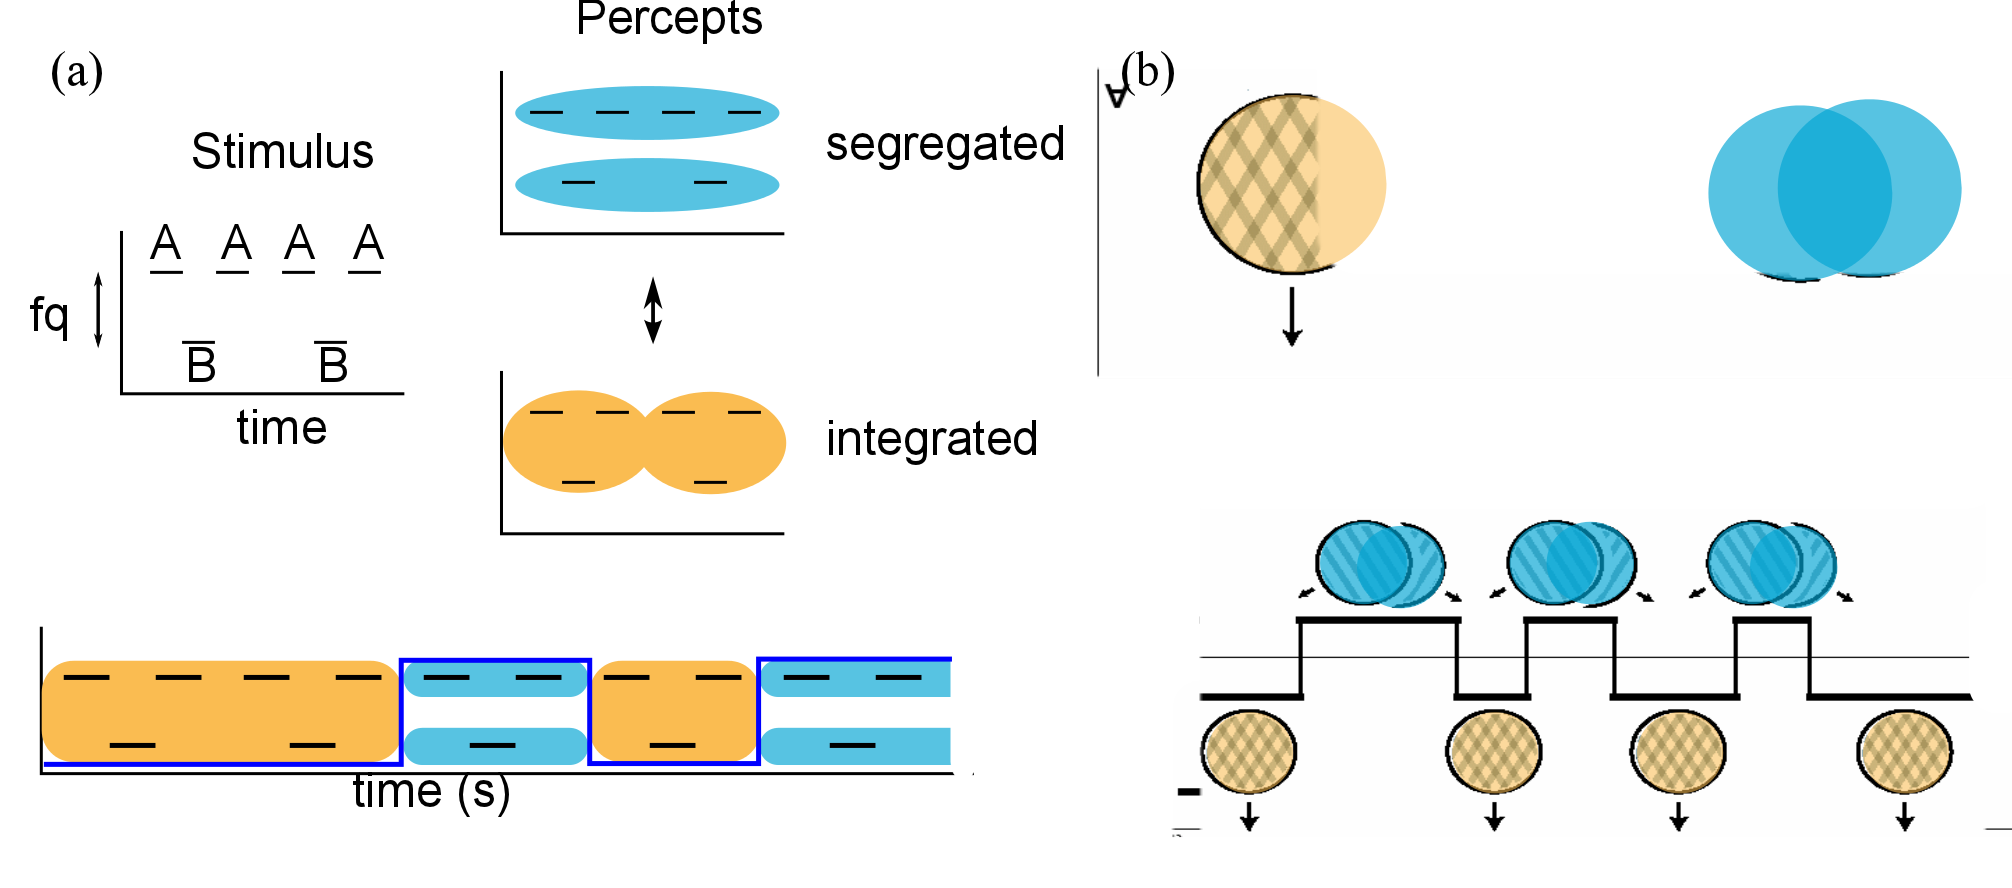
\includegraphics[scale=0.4]{../aba_plaid_stimulus-percepts.png}
	\caption{Examples of stimuli that can produce ambiguous grouping. Left, image adapted from Rubin and Hupe (2004). Moving gratings at certain angles can produce ambiguous motion. Observers report alternations between coherent and transparent motion of the component gratings. Right, van Noorden triplets with ambiguous stream segregation. Listeners report alternations between hearing integration and segregation of the component tone frequencies.}
	\label{fig:percepts_timecourse}
\end{figure}

 %However, we show that this need not be the rule for the neural hardware underlying the subjectively sudden, random switches between perceptual states; instead, 
 
% Gene switching...?

%The process of constructing empirical buildup curves involves the averaging over many trials of the timecourse of a random binary state variable (see Figure 2, blue lines). In our statistical model, the initial state (percept) is fixed, but the dwell time in this state is a random variable characterized by its probability density function. Subsequently the system switches randomly between two states, each of which has its own fixed duration distribution.

The long-term dynamics of perceptual bistability consist of alternations between mutually excusive percepts. The duration histogram of each percept is well-fit by a gamma density \cite{Shpiro2009, Pressnitzer2006}. We believe that the short-term buildup in probability of split percepts, observed when short trial perceptual timecourses are averaged, could reflect the dominance duration distributions observed over long trials. To examine this relationship we use the theoretical framework of an alternating renewal process \cite{}. In this investigation we show that these distributions of percept durations, without any mechanism for accumulation, can account for the experimentally observed dynamics of buildup for a stimulus with ambiguous grouping, as follows:

\begin{enumerate}
\item the perceptual state alternates back and forth between grouped and split
\item the durations for these perceptual epochs are random, independent and stationary
\item the initial percept on a given trial is always the grouped percept
\end{enumerate}

%This theoretical framework ignores history dependence between perceptual epochs and predicts .


\section*{Results}
\subsection*{Alternating renewal process}

The process of constructing empirical buildup curves involves the averaging over many trials of the timecourse of a random binary state variable (see Figure 2, blue lines). In our statistical model, the initial state (percept) is fixed, but the dwell time in this state is a random variable characterized by its probability density function. Subsequently the system switches randomly between two states, each of which has its own fixed duration distribution.

%Thus the perceptual timecourse for a given trial with a fixed stimulus, eg the reports for being in one or the other of the possible perceptual states over time, can be approximated as alternating draws from duration distribution. We model the perceptual durations as being gamma distributed. If we assume that at the beginning of a trial, the first perceptual state will be that of the grouped percept, we can appreciate that buildup is simply the averaging over many trials of random switches out of (as well as back into) a known starting state (Figure 1). This describes an alternating renewal process (ARP).

We initially tested this theory in Monte Carlo simulations by simply constructing in silico perceptual timecourses according to the above assumptions (see Figure \ref{fig:makingBUFs}, (a)). For a given simulated trial timecourse, we draw alternating random samples from each of two distributions-- one corresponding to the grouped state durations, and the other to the split state durations. We begin with the distribution corresponding to the grouped state, and continue drawing samples until the sum of all the durations exceeds the length of a trial. These trial durations are converted into discretized timecourses by assigning a value of 0 to time intervals during which the state corresponds to a grouped percept, and assigning a value of 1 to the time intervals for which the percept state was split. In Monte Carlo, we produce an arbitrarily large number of such trial timecourses, then take the average at each time point. 

\textbf{We have also derived an analytical solution to this process. There are a number of advantages to characterizing the buildup function in this way. First, with an analytical solution relating the distributions of durations for grouped and split percepts to the buildup function, it is theoretically possible to interconvert between buildup functions and the statistics of the dominance durations for each percept. We have developed this solution into a statistical switching model to reconstruct the buildup function from four parameters- the parameters for the gamma densities for grouped and split percepts. This theoretical solution coincides with the Monte Carlo results  (see Figure \ref{fig:makingBUFs}, (b)). This is convenient, as the analytical solution is both computationally less expensive than iterative Monte Carlo simulations, and the solution is exact. Furthermore, in the alternating renewal process framework, there is no need to directly account for any mechanism of accumulation. Therefore, this formulation challenges the conventional understanding of buildup of sound source segregation as a gradual accumulative process.}
	
	
\floatsetup[figure]{style=plain,subcapbesideposition=top}
\begin{figure}
	\centering
	
	  \sidesubfloat[]{\label{fig:a}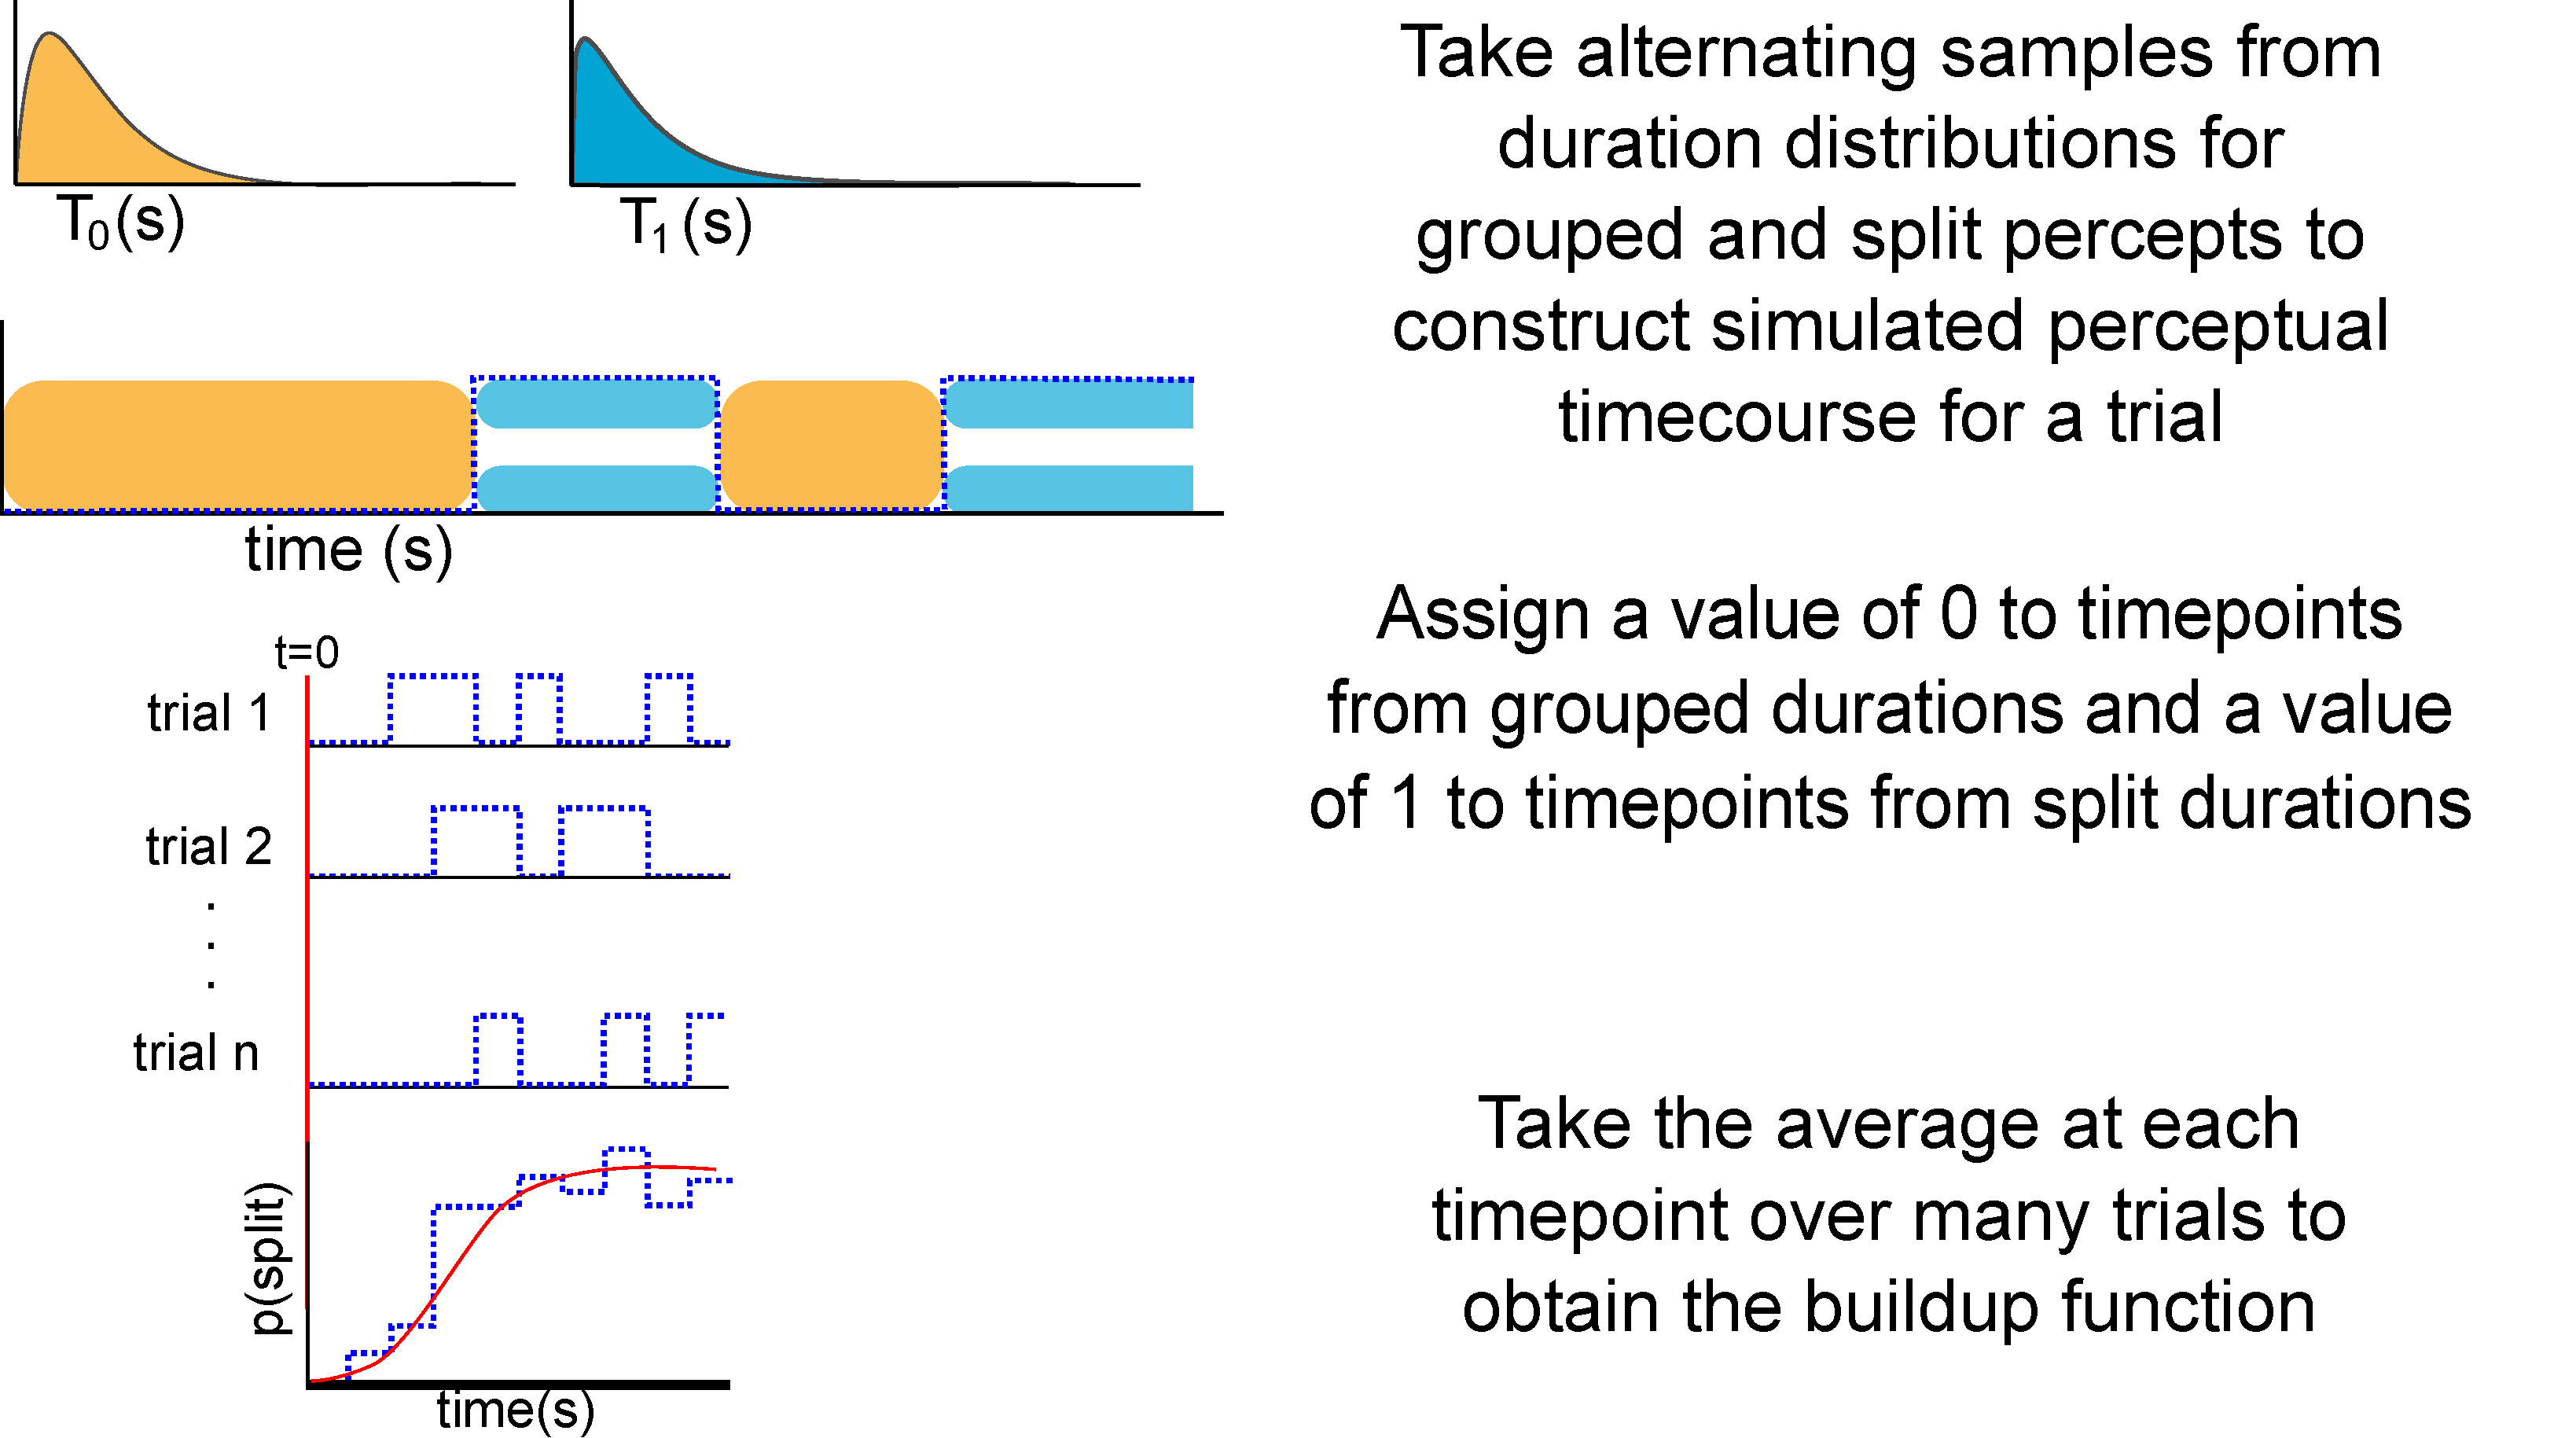
\includegraphics[width=0.65\textwidth]{../percepts&distributions&BUF}} \\
	  \vspace{20 pt}
      \sidesubfloat[]{\label{fig:b}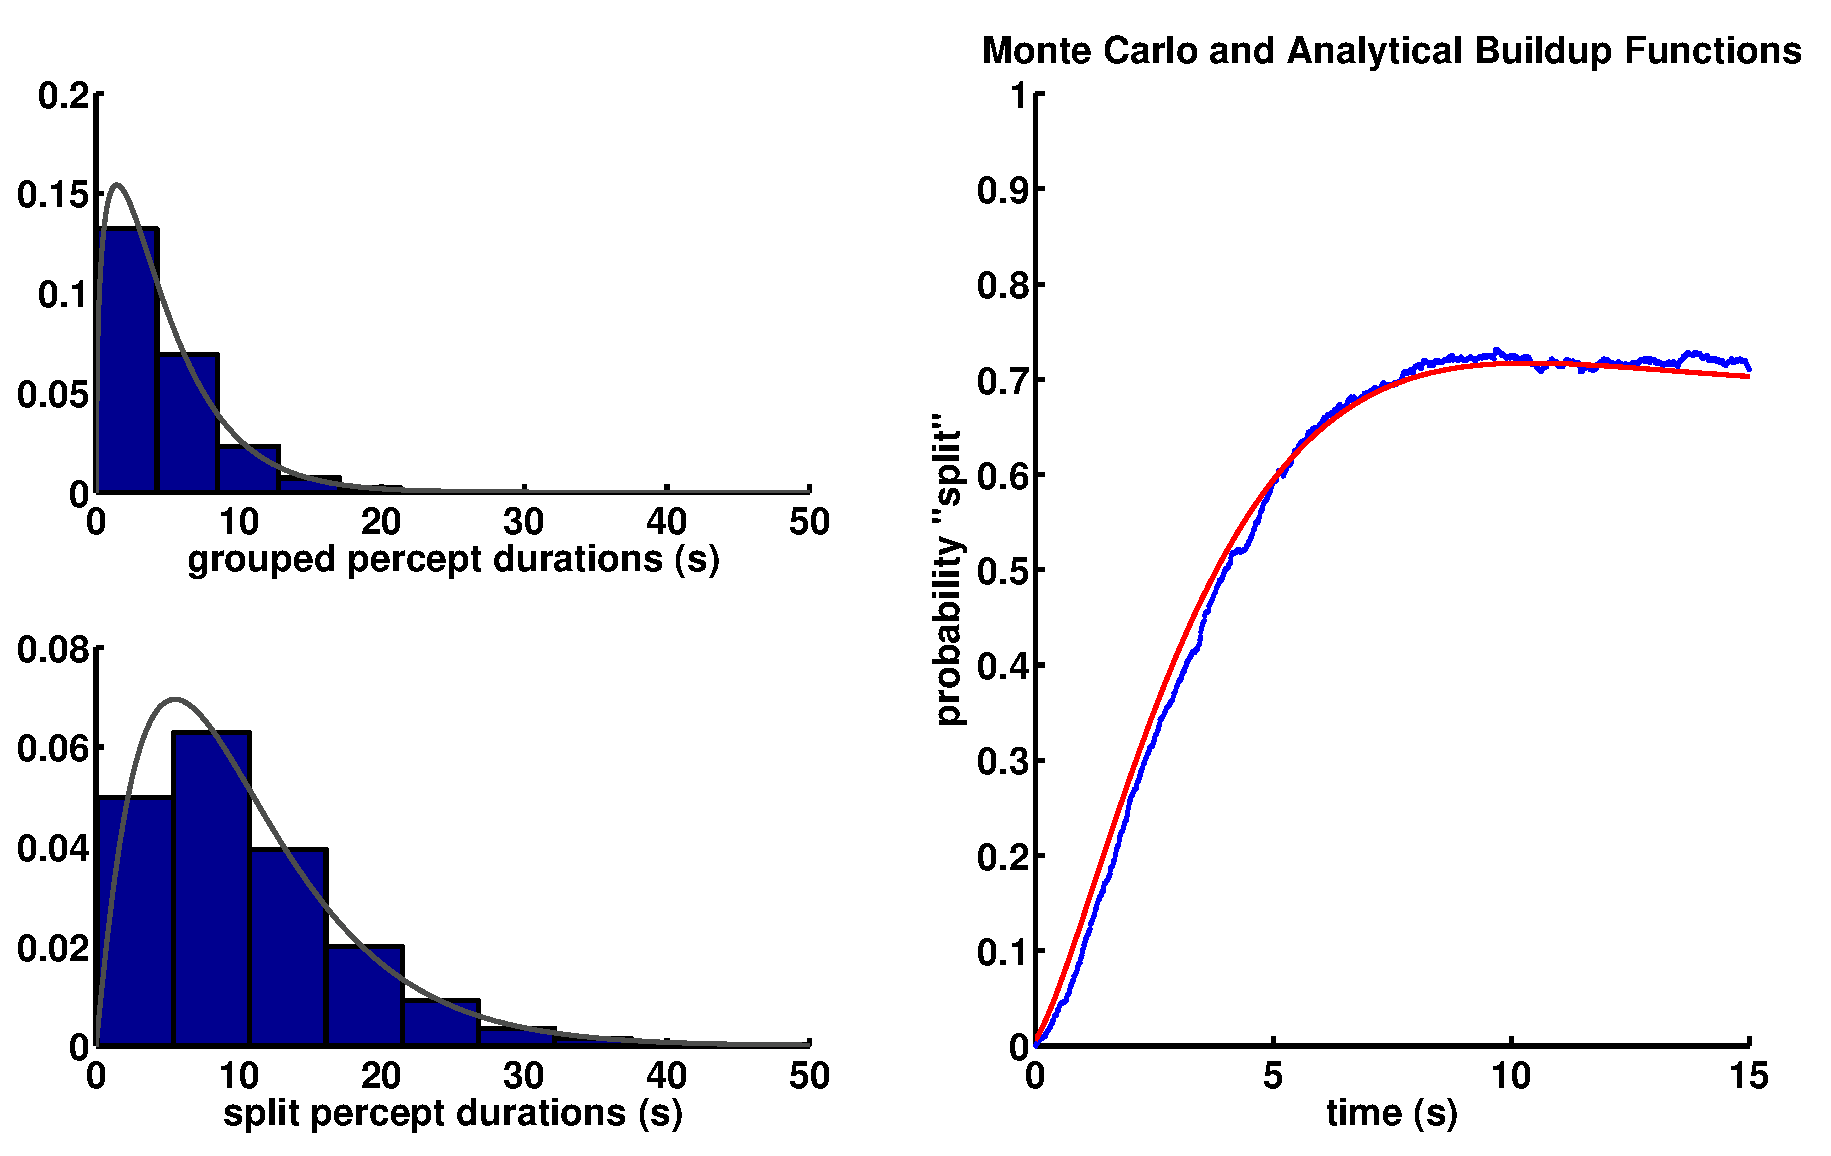
\includegraphics[width=0.7\textwidth]{../monte_carlo_convergence}}
   
 % requires the graphicx package
   %\caption{\textbf{a)} Cochlear spectrogram and \textbf{b)} power spectrum of a harmonically structured synthesized novel sound.}
 
	
	\caption{\textbf{(a)} Visualization of the alternating renewal process producing a buildup function. We used gamma probability density functions approximating duration distributions to construct Monte Carlo simulations. The analytical solution to the alternating renewal process model, shown as a red solid curve (bottom), allows us to predict buildup as a function of the distributions of dominance durations of each of the perceptual states. \textbf{(b)} Monte Carlo computed buildup function of 1000 trials (blue) approaches the theoretical solution (red). Gamma distribution parameters chosen from fits to a preliminary psychophysical dataset (not shown).}
	\label{fig:makingBUFs}
\end{figure}

%We tested whether perceptual bistability models were capable of producing buildup if the starting state was fixed, and under which dynamical regimes.\cite{Shpiro2009}

\subsection*{\emph{Competition model simulations produce buildup as a consequence of alternations}} 

Previous work (Wilson \& Cowan, Laing \& Chow, \cite{Shpiro2009},\cite{Pastukhov2013}) has used population firing rate models with competition architecture to model perceptual bistability. In these pseudoneuronal mutual inhibition models, there are separate populations whose firing rates represent the perceptual strength of each interpretation of the stimulus. These models were originally developed to describe binocular rivalry, but have also been used to account for the psychophysical results of experiments with ambiguous grouping-- namely, moving plaids with coherent/transparent motion (Shpiro, L\&C) and triplets with streaming integration/segregation (Denham?).

In competition models, the relative firing rates of the two populations are taken to produce the simulated observer's perceptual reports. The population with the higher firing rate corresponds to the dominant percept. Because the two populations mutually inhibit each other, in most cases only one population is active at any given time. In addition, each population undergoes adaptation in response to its own firing rate. The alternation of dominance epochs between the two populations can be driven by two mechanisms-- if adaptation is strong enough, then the drive on the dominant population will decay over time, while the suppressed population recovers from any prior adaptation. This leads to periodic alternations between dominance states with oscillation dynamics. However, if adaptation is weak, the system will display attractor dynamics, in which alternations are driven by noise in the externally applied inputs.

The difference between oscillator and attractor dynamics in these competition models is most simply understood by observing how the system would behave without noise \cite{Shpiro2009}, \cite{Moreno-Bote2007}. For oscillation dynamics, slow adaptation would cause the dominant population to reduce its activity over time, reducing the inhibition on the suppressed population, allowing it to become active. In a noiseless system, stable fixed points in the system to appear and disappear over time, and alternations will occur deterministically with a constant period. Noise in such a system will affect the distribution of dominance durations for each state, but is not required for switching. Conversely, attractor dynamics occurs when a system has multiple stable states at the same time. In the absence of noise, the initial conditions determine which state becomes active, and the system behaves in a winner-take-all fashion. That is, the population that becomes dominant first is permanently active, and the other population is permanently suppressed. However, injecting noise into such a system can cause switches from one stable state into another. In this case, the switching between perceptual dominance states would be caused by the noise itself. The brain appears to be a very noisy system, with random fluctuations occurring at multiple scales such as vesicular release and spiking variability.

We wanted to use the competition model as a test-bed for the theory of the alternating renewal process. \textbf{We chose initial conditions that ensured that the grouped percept was always dominant at the beginning of the trial, as our hypothesis that alternations could produce buildup relies on this assumption.} We did this in the simplest manner possible (see Figure \ref{fig:making_comp_BUFs}), by setting the initial condition on the population representing the grouped percept to half its maximum value. All other initial conditions were set to 0. From the population firing rates we computed dominance durations, which were converted to binary timecourses and averaged over trials to produce competition model buildup functions. Using this method, we produced buildup functions for both oscillator and attractor competition models.

To test the application of the alternating renewal process model, we viewed dominance durations of each state from the short simulated trials as samples from underlying gamma distributions. Because our competition model simulations generated trials that were only 20 seconds long, a large proportion of these durations were truncated by the end of the trial. We estimated gamma parameters $k$ and $\theta$ that maximized the likelihood of the complete as well as the right-censored dominance durations for each model "perceptual" state. Using only the four parameters so obtained, we were able to get very strong fits to the buildup function (R-squared $>$ 90\%).


\floatsetup[figure]{style=plain,subcapbesideposition=top}
\begin{figure}
	\centering
	\sidesubfloat[]{\label{fig:a}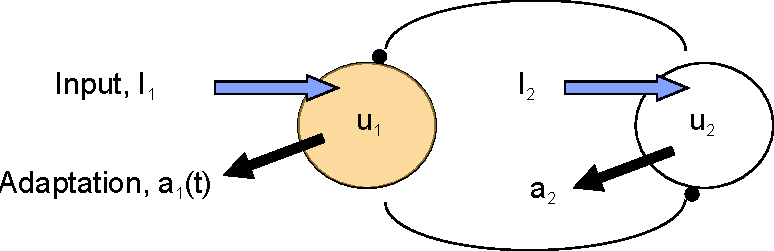
\includegraphics[width=0.6\textwidth]{../comp_model}} \\
	\vspace{20 pt}
	\sidesubfloat[]{\label{fig:b}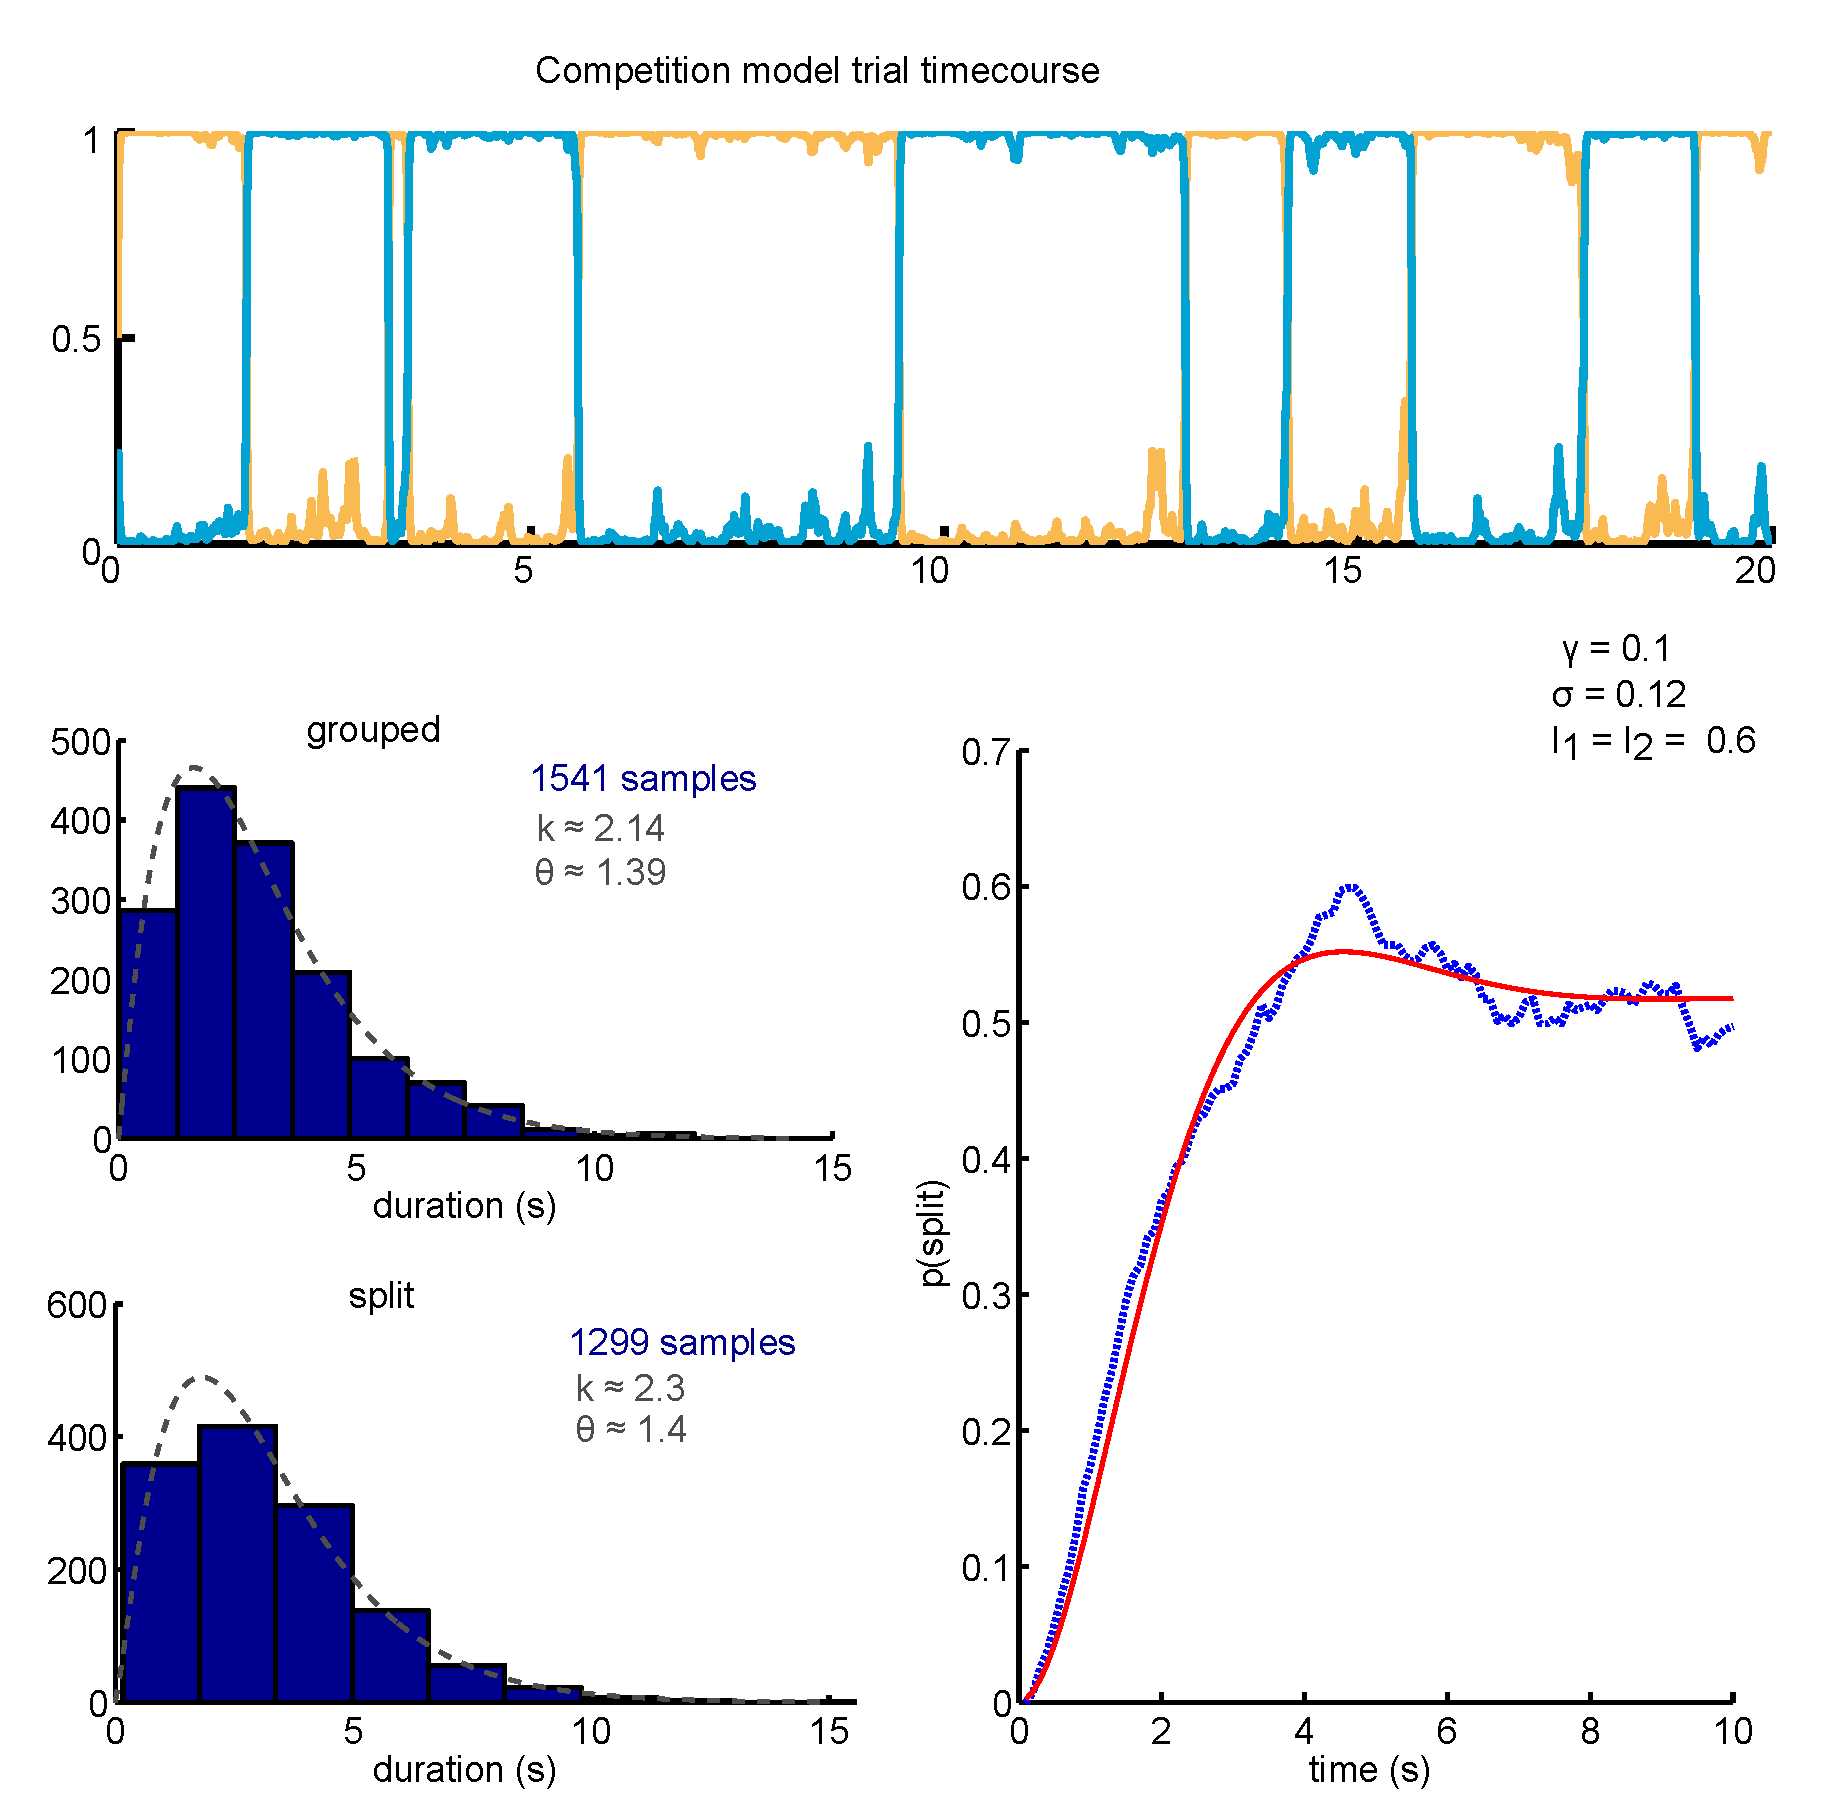
\includegraphics[scale=.45]{BUFs_hists_lowadapt}}
   %\includegraphics[scale=.33]{hi_adapt_low_noise_equal_inputBUFshists} 

   
 % requires the graphicx package
   %\caption{\textbf{a)} Cochlear spectrogram and \textbf{b)} power spectrum of a harmonically structured synthesized novel sound.}
 
	
	\caption{\textbf{(a)} Mutual inhibition population firing rate model producing buildup. Two neural populations $u_1$ and $u_2$, each representing one possible interpretation of a stimulus, are driven by constant external input $I$, representing the external cues in favor of one or another percept. The populations mutually inhibit each other, so that only one can be dominant at a given time. In addition, they each undergo slow spike frequency adaptation. We choose initial conditions to ensure that the population representing the grouped percept, $u_1$, is always dominant at the beginning of a given trial timecourse. \textbf{(b)} Competition model simulation results for parameters that produce attractor dynamics with noise-driven switching. Top, population activity timecourse for one 20-second trial. 500 trials were simulated to produce the buildup function, lower right (blue). Histograms of the dominance durations, with maximum likelihood estimated gamma density parameters, are shown in the lower left. These parameters allow us to compute analytically the resulting buildup function (red).  The buildup function looks similar to those reported in the psychophysical literature, and the ARP prediction is good (R-Squared = 98\%).}
	\label{fig:making_comp_BUFs}
\end{figure}

\subsubsection*{\emph{Psychophysically observed buildup is inconsistent with alternations under oscillation dynamics}}

Previous work from our lab has shown that oscillation dynamics are inconsistent with a number of statistical features of the dominance durations reported in psychophysical experiments \cite{Shpiro2009}. The mean and circular variance of dominance durations under this dynamical regime do not fall within the range of those observed for perceptual reports of ambiguous visual displays. Furthermore, when adaptation drives alternations in the dominance of population activity, we observe moderate and significant correlations between successive percepts. Data from the psychophysical literature suggests that the durations of subsequent percepts are only weakly correlated, if at all \cite{Pressnitzer2006}.

We wanted to examine buildup under each of these dynamical regimes in order to determine whether we could find correspondence between the buildup functions produced by competition models and those reported in the psychophysical literature. Previously reported psychophysical data suggest that buildup is largely a monotonic proess. To our knowledge, no psychophysical experiments have shown a buildup timecourse with a damped oscillatory approach to steady state. Buildup functions produced under oscillation dynamics in our competition model (Figure \ref{oscillation_dynamic_buildup}), however, display damped oscillations reflecting the underlying periodicity of the mechanism of alternation. % If buildup is a consequence of alternation between states, then those alternations are probably not the result of an oscillatory process.

Alternations with attractor dynamics, however, produce buildup functions that are mostly monotonic. By computing the buildup function produced under different dynamical regimes, we find converging evidence with previous studies that distinguish attractor dynamics from oscillation dynamics-- when the competition model operates with oscillation dynamics, the buildup function is inconsistent with psychophysically observed buildup functions. 

\begin{figure}
		\centering
		
		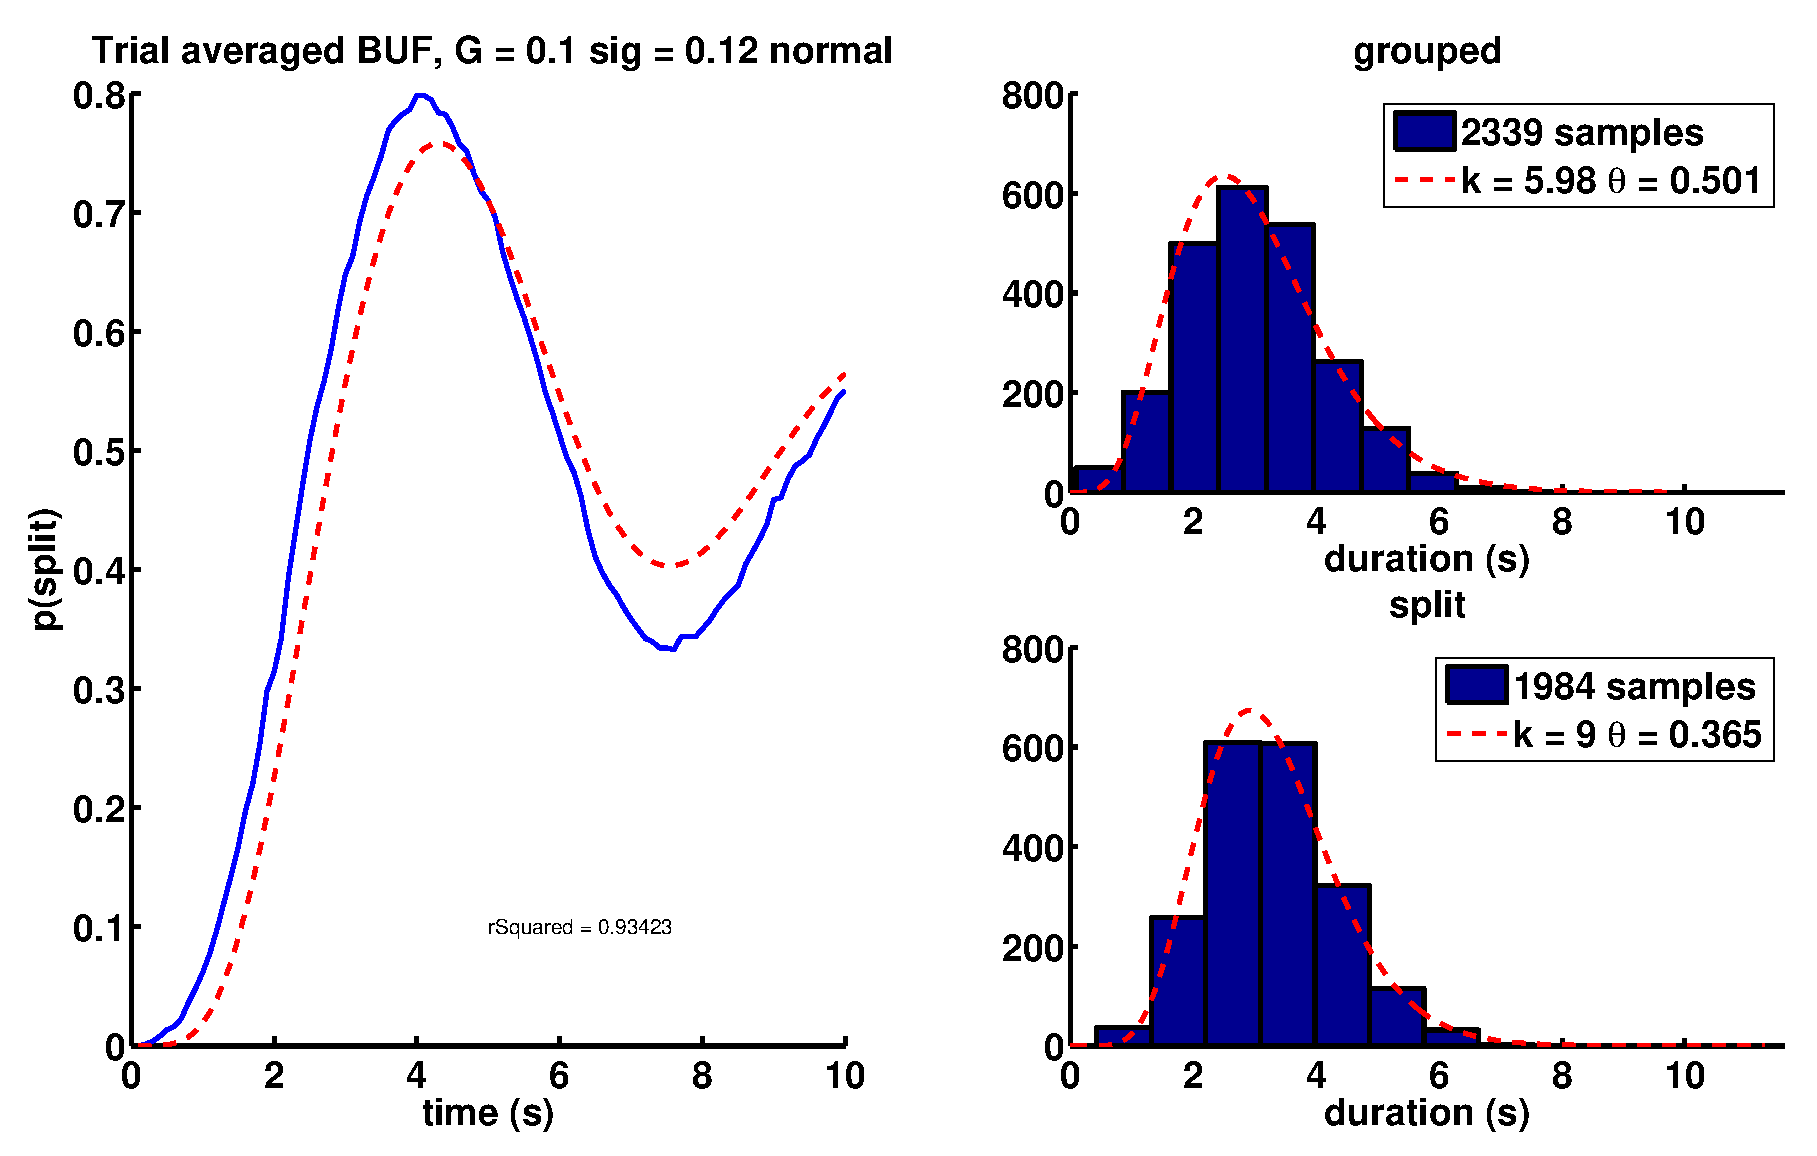
\includegraphics[scale=.45]{hi_adapt_low_noise_equal_inputBUFsHists}
				
		
		\caption{Competition model simulation of buildup under oscillation dynamics, for which switches between dominance states are driven by adaptation. Top, an example trial timecourse. The dominance durations are much more regularly timed, reflecting the clock-like periodicity of the underlying oscillator. These oscillations are dramatically present in the average. The prediction under the alternation hypothesis from the gamma parameters is still quite good (R-squared = 93\%).}
		\label{oscillation_dynamic_buildup}
\end{figure}
		

% Results and Discussion can be combined.


%We hypothesized that buildup would occur within a system that exhibited alternations with a fixed starting state, and used existing dynamical models to try to reproduce the kind of buildup curves seen psychophysically. In particular, previous work has shown that competition models (Wilson \& Cowan, Laing \& Chow) that reproduce the population activity subserving perceptual bistability should have a noise-driven alternation mechanism, rather than operating in an oscillatory regime with adaptation-driven alternations \cite{Shpiro2009},\cite{Pastukhov2013}. This conclusion is based on the statistics of the dominance durations-- to match the mean, circular variance, and history-dependence of human perceptual data, competition models cannot be operating within the oscillatory dynamical regime.

%We used the competition model architecture as a test-bed for our statistical switching model. We wanted to see what buildup functions using parameters that were plausible, according to previous studies, could be differentiated from those which were generated under parameter regimes producing unreasonable dominance duration statistics. We were particularly interested in whether history dependence, in the form of percept-to-percept correlations, would affect the quality of the fits under our statistical model, as it was developed under the assumption of independence between the duration distributions.
%
%\begin{figure}[scale = .5]
%   \begin{center}
%   
%   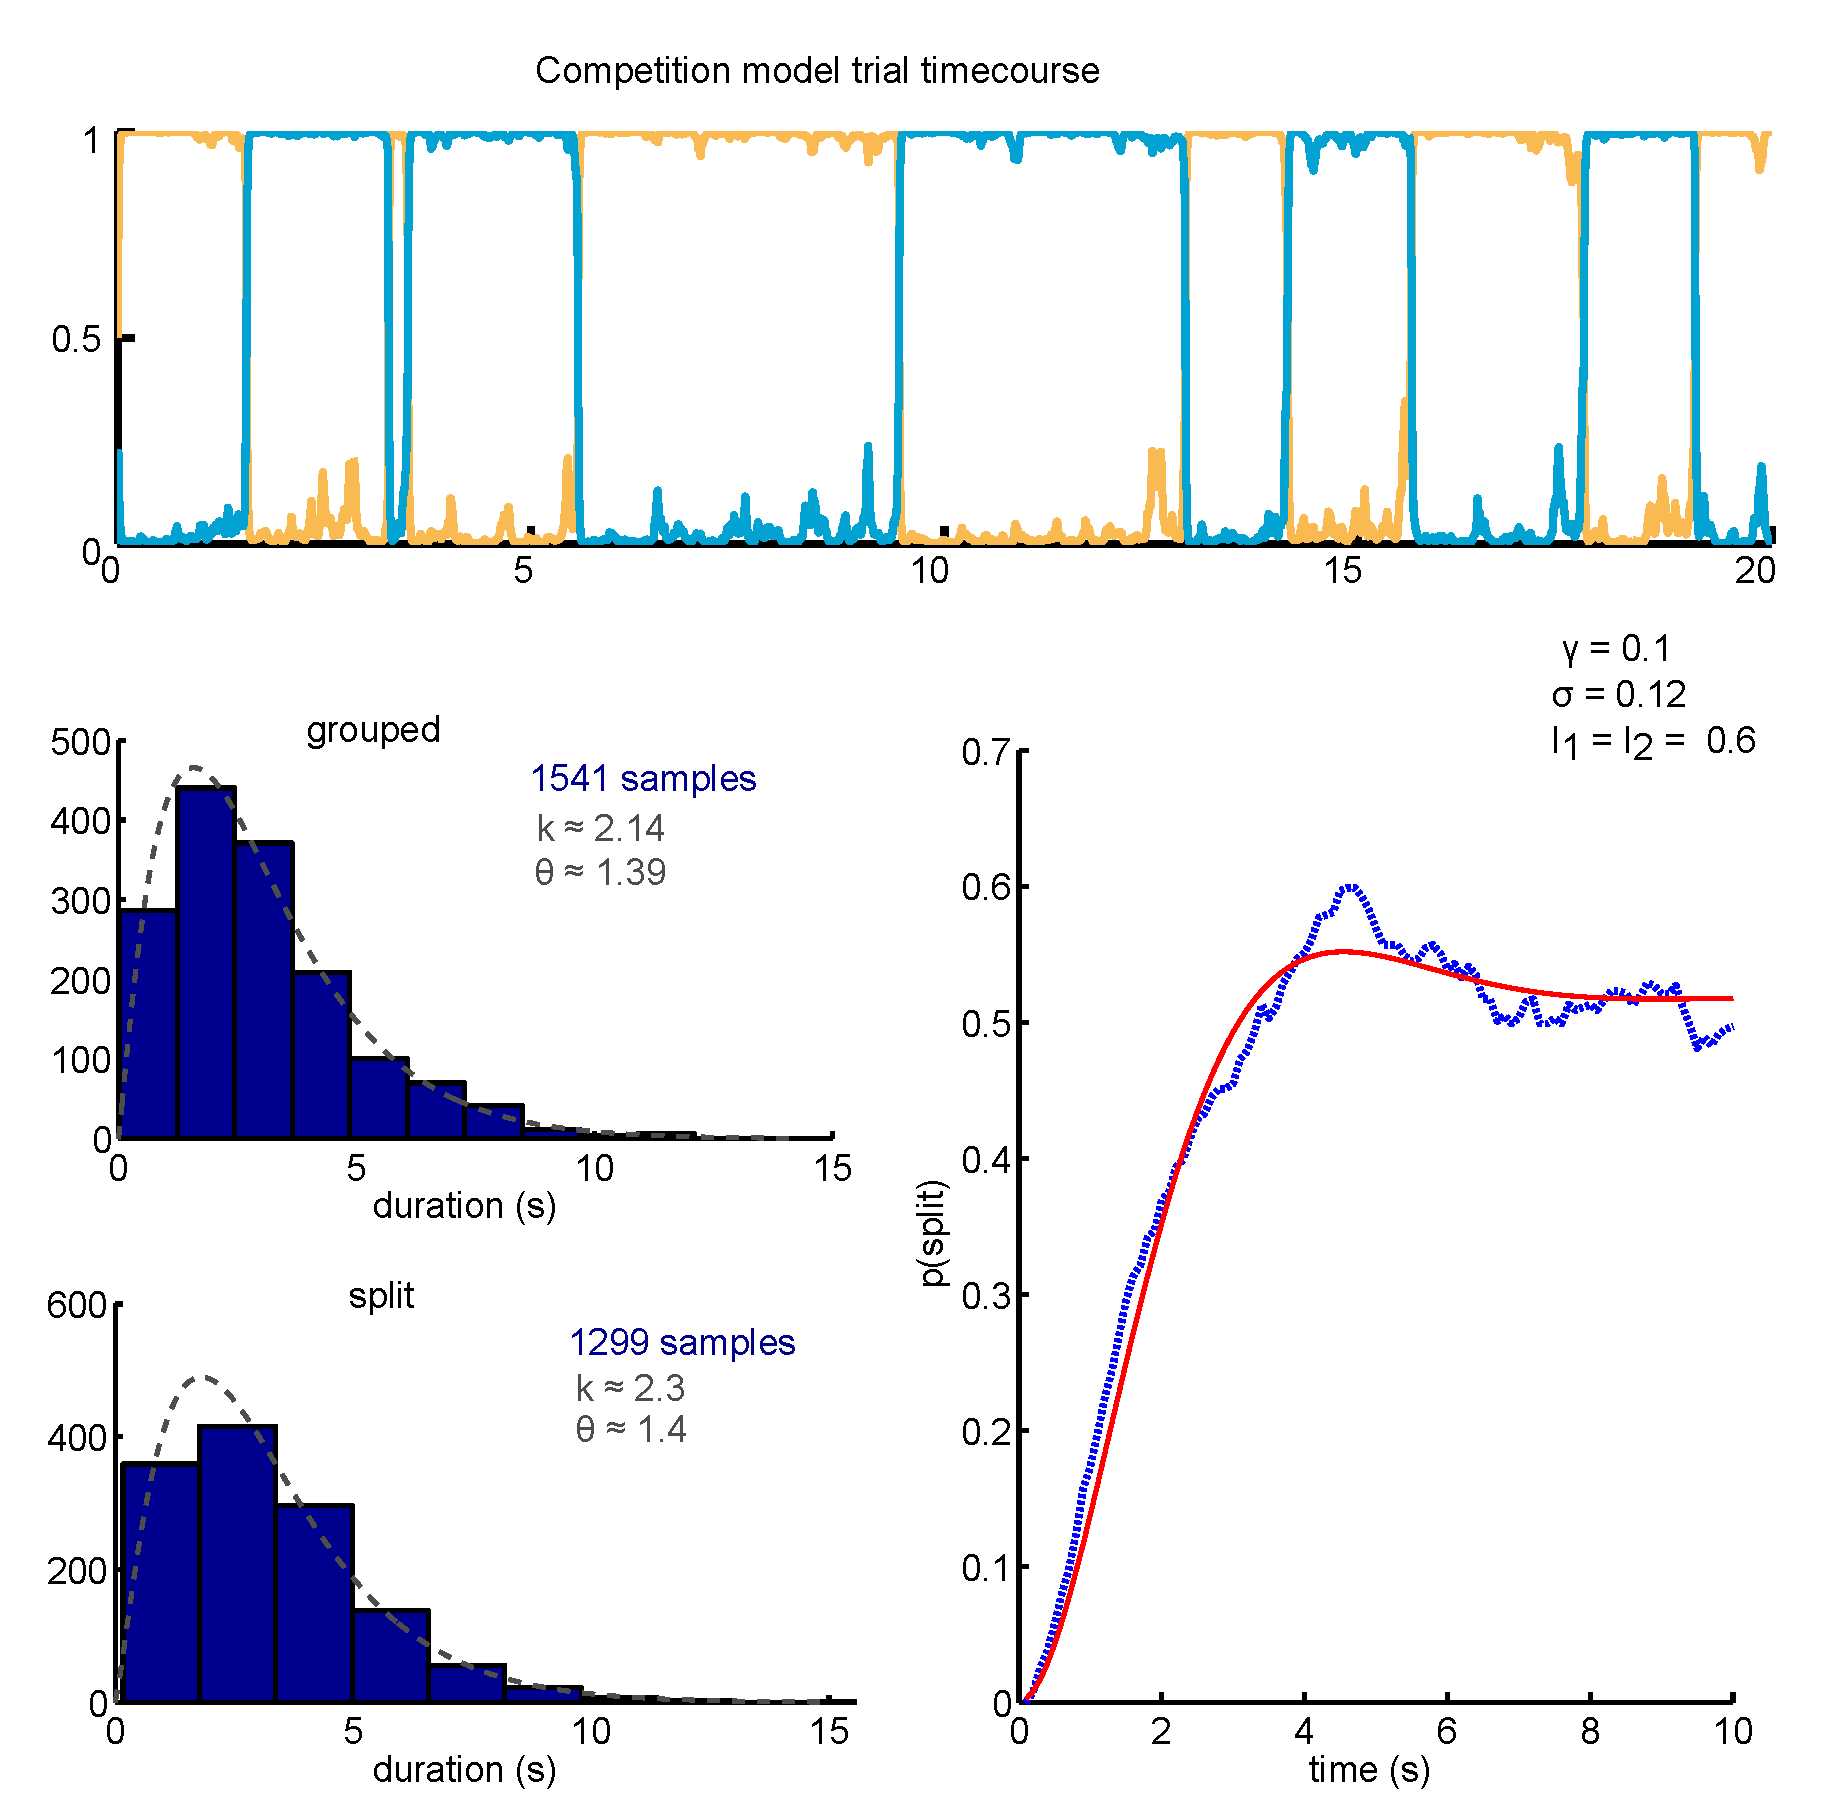
\includegraphics[scale=.45]{BUFs_hists_lowadapt}  
%   %\includegraphics[scale=.33]{hi_adapt_low_noise_equal_inputBUFshists}      
%   \caption{Competition model simulation results for parameters that produce attractor dynamics with noise-driven switching. Top, population activity timecourse for one 20-second trial. 500 trials were simulated to produce buildup function, lower right (blue). Histograms of the dominance durations, with maximum likelihood estimated gamma parameters, are shown in the lower left. These parameters provide the alternating renewal process prediction of the buildup function, plotted in red against the trial average. The buildup function looks similar to those reported in the psychophysical literature, and the ARP prediction is good.}
%   	\label{fig:low_adapt}
%   \end{center}
%\end{figure}


%The results of our buildup simulations provide converging evidence that the alternations cannot be driven by oscillation dynamics (See Figure \ref{fig:mono_vs_periodic}). Noise driven switching is necessary for buildup functions that look like those presented in the literature. In principle, the apparent monotonically increasing likelihood of split percepts over time could also be accomplished by averaging together the timecourses of multiple oscillators with different periods. However, there have been no reports whatsoever of oscillatory buildup functions.





\section*{Discussion}

\subsection*{Do percept-to-percept correlations matter for describing buildup in an alternating renewal process?}

The previous competition model simulations provide a test-bed for our novel statistical model. When given dominance durations are not statistically independent, and there is history dependence between successive perceptual epochs, can the alternating renewal process theory still relate buildup to the underlying duration distributions? We measured the correlations in the data produced for noise-driven and adaptation-driven alternations. As previously reported, the adaptation-driven perceptual timecourses showed moderate correlations between the durations of successive percepts. Our statistical model, however, ignores this history dependence entirely, treating the distributions of percept durations as entirely independent. 

Importantly, even for adaptation-driven switching, for which history dependence between successive durations is prominent (r value of 0.23), the buildup function predicted by the alternating renewal process without any consideration for correlations matched the competition model simulated buildup function with a coefficient of determination of 93\%. We believe that the failure of history dependence to affect the dynamics of buildup results from the loss of information about individual trial timecourses caused by averaging. While the correlations between perceptual epochs may be important for understanding the timecourse of a particular trial, the correlations between specific perceptual epochs are "washed out" by taking the average of many timecourses. Therefore, the dynamics of buildup can be described purely by the underlying distributions of dominance durations.


%The observation that the accumulation of adaptation does not drive the switching between grouped and split perceptual states, and that the buildup function can be predicted from long-term state distributions without any consideration for history dependence between states, may come to some as surprising.
Previous accounts of buildup \cite{Micheyl2005}\cite{Pressnitzer2008} have pointed to the accumulation of adaptation as a critical feature for the switch from a grouped to a split percept. Indeed, multi-second habituation in the auditory periphery \cite{Pressnitzer2008} can predict the behavioral buildup of streaming. It may therefore be surprising that the alternating renewal process neglects to account for adaptation entirely. We believe that previous observations and our own can be reconciled, and may even be complementary. Previous work provides some account for how the switch from the grouped to the split percept might be accomplished as a result of an accumulation of adaptation. While we do not explicity invoke an accumulative process to describe this switch, the use of a gamma density to describe the distribution of dominance durations for the grouped percept implies history dependence. This is because the hazard function for a gamma density, in contrast to an exponential distribution, is dependent on time elapsed, evolving from 0 at time zero to a steady state value. The time dependence of the probability of switching out of the grouped percept may therefore be complementary with previous descriptions. What is still missing from these theories, however, is the mechanism by which the perceptual state switches back and undergoes alternations; how do we account for switches out of the split percept, and the distribution of split durations?

\subsection*{Duration distributions are not well constrained by the trial average}
The resilience of the alternating renewal process to capture the dynamics of buildup in a variety of circumstances, including those with duration-to-duration correlations likely carries the burden of overflexibility-- for any given buildup function, a wide range of pairs of distribution functions may provide a good fit. We generated buildup functions using Monte Carlo as in figure \ref{fig:makingBUFs} and used our analytical solution to find the gamma density parameters that minimized the squared error between the Monte Carlo and analytical buildup functions. In general, the parameters so found did not strongly fit the histograms of the duration samples used (see Figure \ref{reverse_fit}). Specifically, whereas maximum likelihood confidence intervals estimated from the duration samples generated to construct short trials always contained the parameters to the gamma densities used in the Monte Carlo random number generators, the least squares estimates to the buildup function were only within the confidence intervals from the maximum likelihood estimates\textbf{for 1 in 10 simulations}.

\begin{figure}
	\centering
	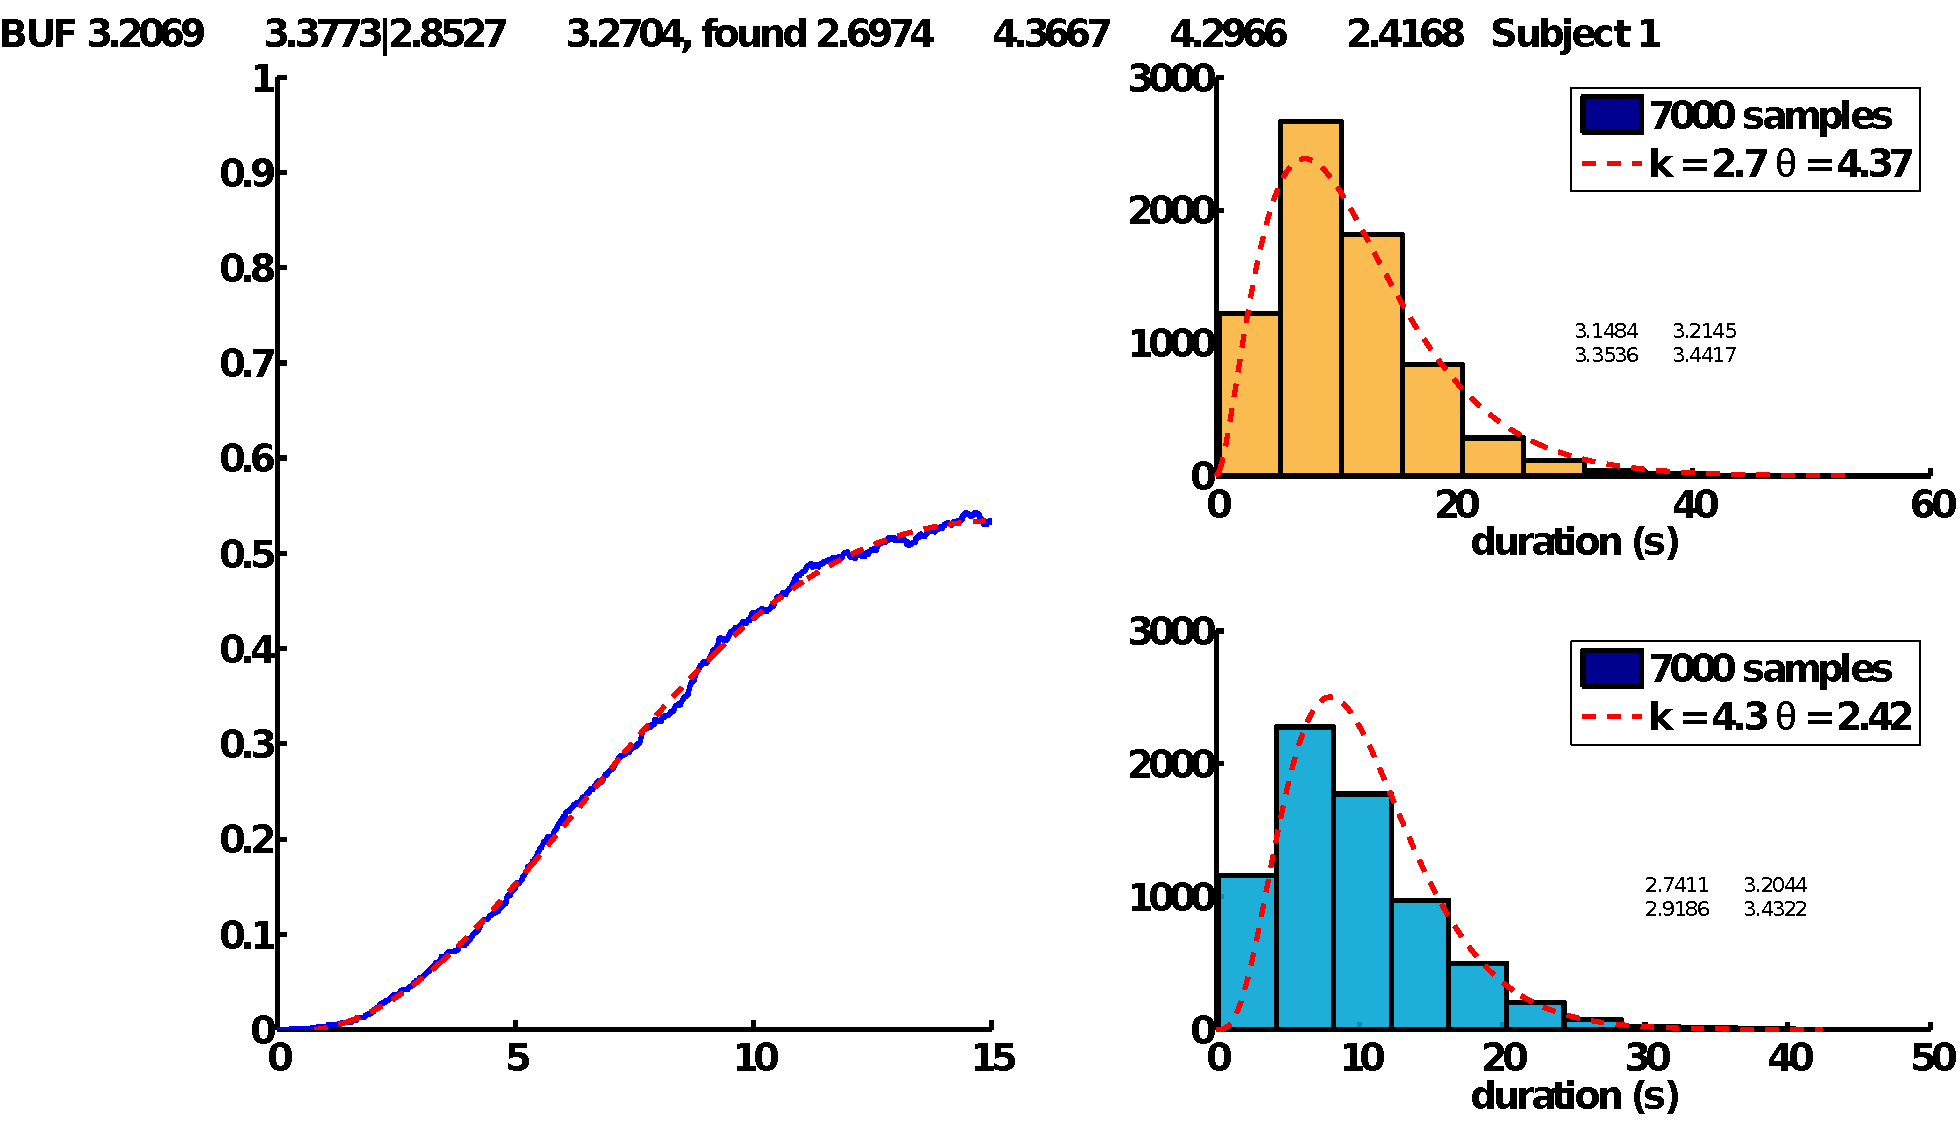
\includegraphics[scale=.45]{../reverse_fit1}
	\caption{}
	\label{fig:reverse_fit}
\end{figure}

\textbf{However, for the special case when the both perceptual states have identical duration distributions, the parameter estimation for the gamma density functions from the buildup function is much better. This circumstance would occur when the inputs to the populations representing each percept are matched, e.g., when the stimulus is perfectly ambiguous. We generated buildup functions using Monte Carlo from two identical gamma densities, and found the single set of gamma parameters that minimized squared error between this and theoretical buildup function. For 1000 such simulations, 24.75\% of the recovered parameters were within maximum likelihood confidence intervals, and in general the fits were much closer. For instances in which the original data (trial timecourses and durations) are unavailable, this method of estimation may prove useful for providing at least a rough estimate of the duration distributions underlying long-term dynamics.}

\begin{figure}
	\centering
	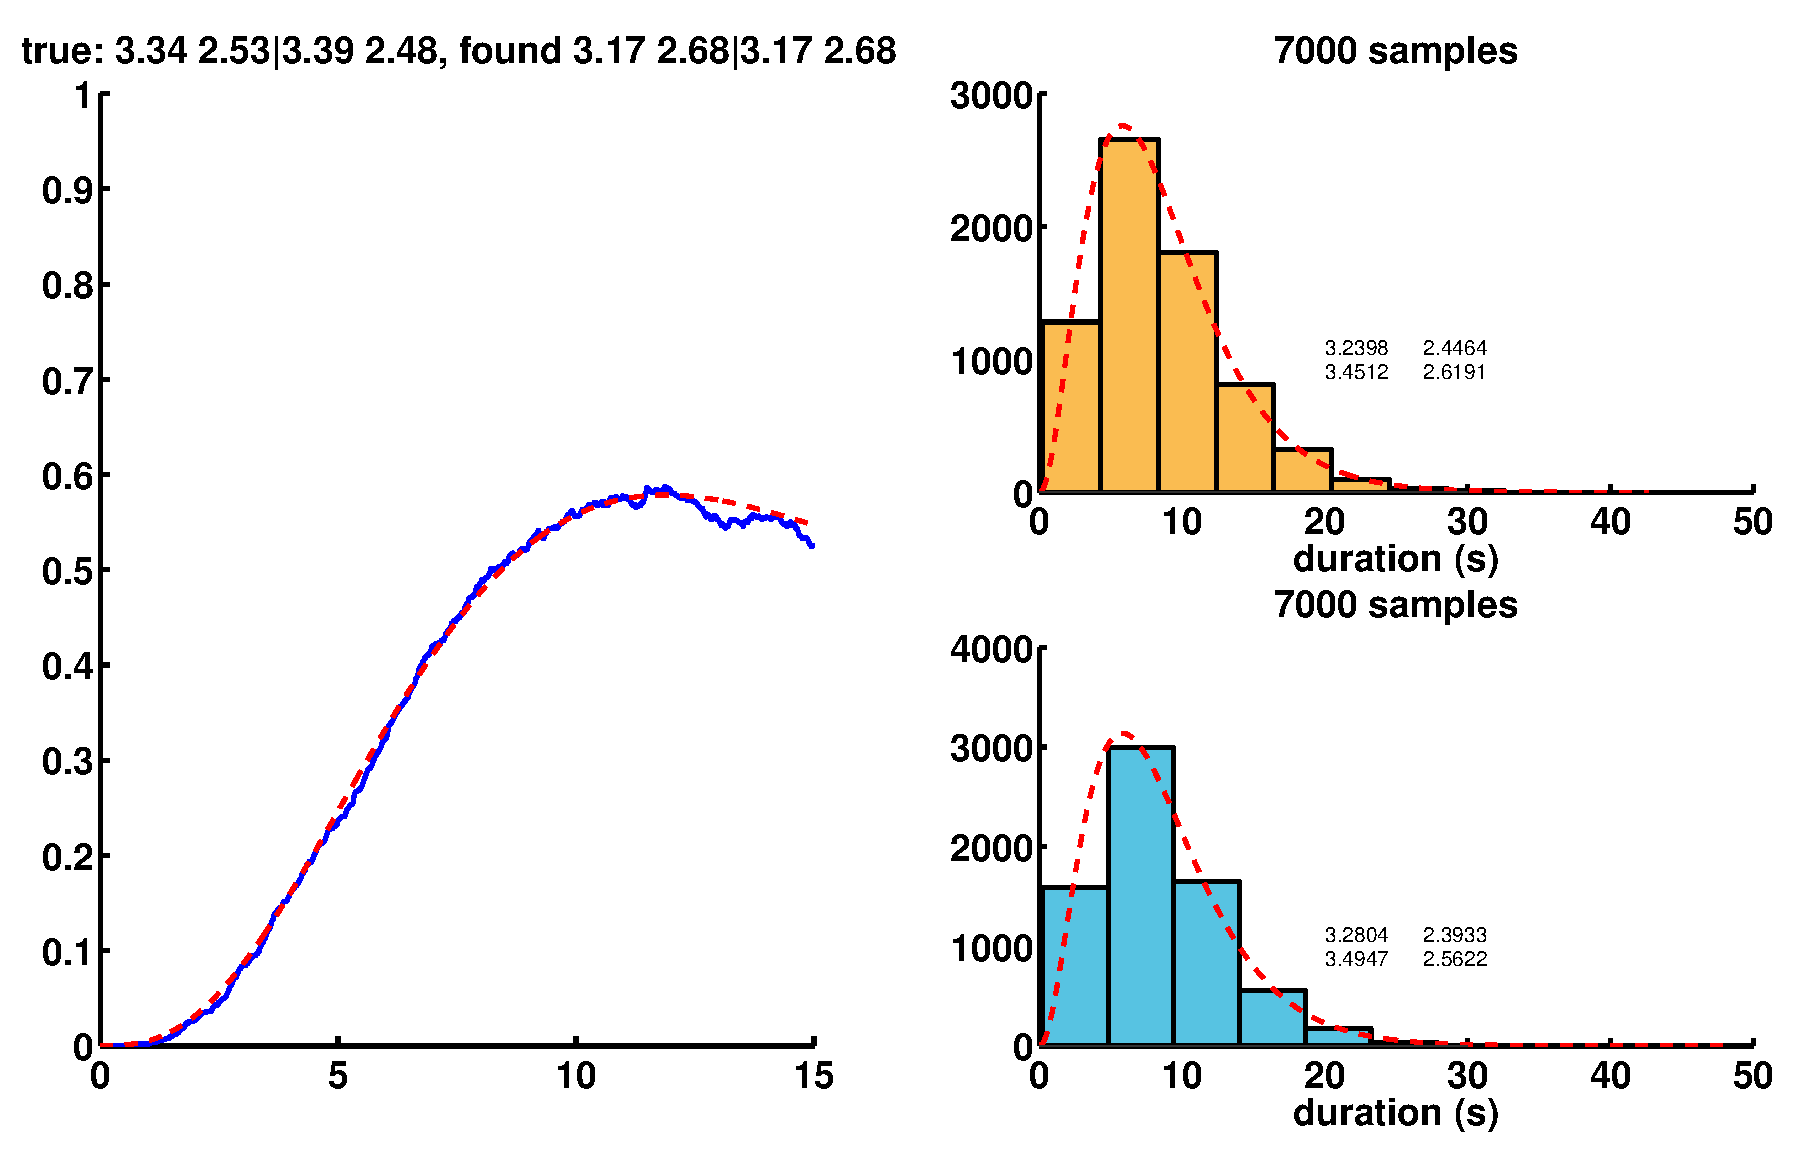
\includegraphics[scale=.45]{../2parReverseFits/ex1}
	\caption{Better with 2 par model}
	\label{fig:2par_reverse_fit}
\end{figure}


 % In addition, there may be special cases-- such as when one can assume that the distributions are identical, as may be the case for competition model simulations with the same external input to each population-- for which the parameter estimates are better constrained.

\subsection*{What if the first percept is longer?}
\textbf{One issue we have not addressed so far in our presentation of the alternating renewal process model is inertia \cite{Hupe2012}. For ambiguous displays, the time until the first perceptual switch is typically much longer than subsequent durations of the same percept. For stimuli with ambiguous grouping, the distribution of initial grouped percept durations is different from other grouped percepts. Our theoretical model is capable of computing the buildup function from both steady state and initial percept distributions; however, this would introduce a third duration distribution, and increase the number of parameters to 6. For simplicity's sake, we have only shown the 4 parameter model, which assumes that the initial percept duration is drawn from the same distribution as other grouped percept durations.}

\textbf{Our competition model, as it stands, produces a different distribution for initial and subsequent grouped percepts. However, the initial percepts are shorter in mean duration. This can probably be fixed by using a different set of initial conditions to achieve the correct initial dominance state-- for instance, by setting the initial conditions so that the other population, that which represents the split percept, is highly adapted at the beginning of the trial. However, such an approach would be arbitrary, and leaves something to be desired in terms of explanatory value. What would be better is a more detailed model that captures elements of the sensory coding and neural dynamics that produce the perceptual states in the first place. For instance, percept formation might be subserved by neural populations that respond only to particular spectrotemporal input patterns. These encoding neural populations would be subject to adaptation, etc, and could allow us to make predictions about the perception of novel stimuli.}
%First, address the adaptation initial condition. This isn't as desirable because it is still completely arbitrary. Would be better to have a more detailed explanation with sensory coding rationale, neurophysiology. So future directions are to make a model that produces fixed first percepts more reasonably.

\textbf{Our theoretical solution can be modified to account for experimental data in which the initial percept duration distribution is different from the steady state. However, there are circumstances in which inertia is fairly trivial, such as when buildup resets after a switch in attention \cite{Denham2010}. Stationary distributions might be appropriate for such circumstances. We can take a more abstract view and consider a steady-state buildup function constructed from averaging over timepoints aligned by switches into the grouped percept.}

\subsection*{Switch-triggered averaging produces steady state buildup function}

\textbf{To address the issue of inertia and the longer mean duration of the initial percept than subsequent grouped percepts on a trial, we explored a new method for constructing the buildup function: switch-triggered averaging. This method allows us to produce a buildup function from a single long trial. Ignoring the first and second percept duration, we constructed buildup functions by estimating the probability over time for the split percept based on an event-triggered average aligned to each switch into the grouped percept. This method produces a buildup function at steady state, the probability of perceiving the split organization not just from the beginning of the trial but rather from the beginning of any grouped percept duration over the course of a long presentation.} %This type of buildup function will draw from the stationary distributions of percept durations.}

\subsection*{Summary}






%\subsection*{Ambiguity}
%The time it takes to achieve the steady state fractional dominance ratio should depend on both how far the original fractional dominance ratio from the steady state as well as the strength of the biasing input in favor of either of the two states. In Figure \ref{fig:ambiguous_vs_biased} we see that the strength of the biasing input is much more important to defining the overall timescale of buildup than the distance between starting and steady states. This effect is in contrast to the effect on mean durations; mean durations for grouped percepts in the ambiguous case was 8.07 s, and for split 7.57 (grand mean =  7.8) whereas for the biased case, the average grouped duration was 1.29 s, the averaged split duration was 18.213, and the grand mean was 9.75. So while switches occurred more frequently in the ambiguous case, the time to half-maximum was also longer.

%\begin{figure}[scale = 1]
%   \begin{center}
%   
%   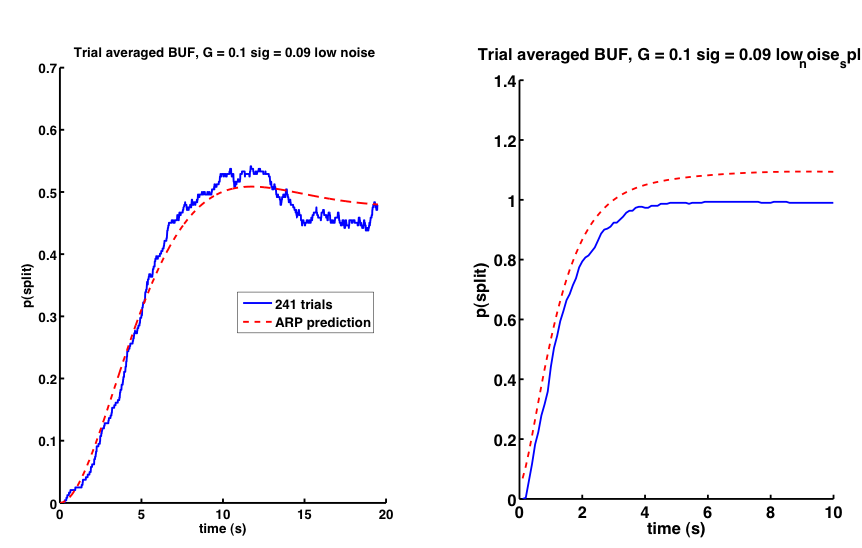
\includegraphics[scale=0.33]{../ambiguous_vs_biased}
%   
%   \caption{When stimulus is very ambiguous, leading to steady state equal fractional dominance durations, buildup is slow-- left, half-maximum is achieved after about 5 s. However when the stimulus is strongly biased, the steady state is achieved in much shorter time (~2s), even when this is further from the starting state.}
%   	\label{fig:ambiguous_vs_biased}
%   \end{center}
%\end{figure}
%%
%\newpage
%\newpage
%\section*{Discussion}
%
%These results support the growing body of research suggesting that accumulation of adaptation is not the primary cause of alternations \cite{Pastukhov2013}. In addition, recent research has suggested that the transient phenomenon buildup is only truly present in displays that elicit perceptual alternations in observers with long presentations \cite{Deike2012}. (BUT ARE THERE EXPERIMENTS IN WHICH BUILDUP IS OBSERVED FOR SOME NON-AMBIGUOUS STIMULUS? DOES BUILDUP EXIST FOR NON ABA STIMULI, BECAUSE THAT'S WHY IT'S APPEALING AND ANY STIMULUS THAT SHOWS BUILDUP MIGHT BE USEFUL FOR ALTERNATION)

% You may title this section "Methods" or "Models". 
% "Models" is not a valid title for PLoS ONE authors. However, PLoS ONE
% authors may use "Analysis" 
\section*{Methods}
\subsection*{Competition model simulations}
Competition model simulations followed the procedures reported previously in \cite{Shpiro2009} for population firing rate model with spike frequency adaptation. Specifically,

\begin{equation*}
	\begin{cases}
	\dot{u}_1 & = -u_1 +  f(-\beta u_2 - \gamma a_1 + I_1 + n_1) \\
	\tau_a \dot{a}_1 & = -a_1 + u_1\\
	\dot{n}_1 & = \frac{-n_1}{\tau_n} + \sigma \sqrt{\frac{2}{\tau_n}} \eta(t)\\
	\dot{u}_2 & = -u_2 +  f(-\beta u_1 - \gamma a_2 + I_2 + n_2) \\
	\tau_a \dot{a}_2 & = -a_2 + u_2\\
	\dot{n}_2 & = \frac{-n_2}{\tau_n } + \sigma \sqrt{\frac{2}{\tau_n}} \eta(t)
	
	\end{cases}
\end{equation*}

The variable $u_1$ corresponding to the short-time averaged firing rate of the population representing the ``grouped" perceptual state, and $u_2$ the firing rate of the population representing the ``split" perceptual state. The variables $a_1$ and $a_2$ represent the spike-frequency adaptation. Parameter $\gamma$ controls the strength of the adaptation, and $\beta$ controls the strength of suppression from the competing population. $I_1$ and $I_2$ are the external inputs driving the two populations, and $n_1$ and $n_2$ are independent Ornstein-Uhlenback noise generators with mean zero and variance $\sigma$, and a timescale of $\tau_n$. 
The input-output function used was a sigmoid, with $f (x) = 1/(1 + exp(−(x − \theta )/ k))$. 

The simulation was carried out in nondimensionalized time, with the convention that one unit of time corresponds to 10 msec. Time constants given in simulation time units were $\tau_a = 200, \tau_n = 10$. The following parameter values are used: $k = 0.1, \theta = 0, \beta = 1$.  The values of the external inputs to the populations $I_1$ and $I_2$, the adaptation gain $\gamma$ and the noise strength $\sigma$ were varied as specified in the text, with the value of $\sigma$ scaled in relation to the integration time step by $1/\sqrt{dt}$ to keep specified variance per unit time. Simulations were implemented in MATLAB using forward Euler integration with a time step of 0.1 (1 msec real time).

For each combination of parameter values, we simulated 500 trials of length 10 s with initial conditions $u_2(0), a_1(0), a_2(0), n_1(0), n_2(0) = 0$ and $u_1(0) = 0.5$; thus, at the beginning of each simulated trial, the first population to become dominant was always that corresonding to the first percept. With the resulting population firing rate timecourses, we obtained dominance durations by finding time points of the zero crossings of the differences of the firing rates. Using the samples of dominance durations obtained for each population (over 1000 durations for each population with each parameter set), we fitted gamma densities using maximum likelihood estimation. Simulated experimental buildup curves were constructed by averaging across trials the binary timecourse $u_2 > u_1$. 

\subsection*{Derivation for alternating renewal process}
In the alternating renewal process there are 2 random variables, S(t) and Z(t). S(t) is the random elapsed time since last switching into the current state, evaluated at time t. Z(t) is a dichotomous random variable, where Z(t) in ${0,1}$ codes for the percept, grouped or split. For sake of convenience, we introduce 2 probability density -mass functions: $f_0(s,t) ds = Pr \lbrace S(t) \rbrace$ in $(s,s+dt)$ and $Z(t)=0$, and $f_1(s,t) ds= Pr(S(t)$ in $(s,s+ds)$ and $Z(t)=1$. The coupled pair of partial differential equations describing the evolution over time of these 2 probability density-mass functions is as follows:
%The solution to the alternating renewal process was implemented by solving a set of probabilistic differential equations describing the rate of change in probability per unit time for each of the two states of a dichotomous random variable $Z(t) = {0 , 1} $, as follows:

\begin{equation}
\frac{\partial f_0}{\partial t} \big(s,t\big) = -\frac{\partial}{\partial s}\big(1 * f_0(s,t)\big) - h_{T_0}(s) f_0(s,t)
\end{equation}

\begin{equation}
\frac{\partial f_1}{\partial t} \big(s,t\big) = -\frac{\partial}{\partial s} \big(1 * f_1(s,t)\big) - h_{T_1}(s) f_1(s,t)
\end{equation}

where $s$ is the elapsed time since entering state $i$ and $h_{T_i}(s)$ is the hazard function, the probability per unit time of exiting the current state at time $t$. $h_{T_i}(s) = \dfrac{f_{T_i}}{\hat{F}_{T_i}}$, the ratio of the density function of durations $T_i$ for state i and its complementary cumulative distribution function.

The value of $S(t)$ is reset to 0 whenever an alternation between states occurs. The initial flux of probability (a source) at s = 0 is determined by the probability of switches out of the previous state, leading to the following boundary conditions:

\begin{equation}
f_0(0,t) = \int_0^\infty h_{T_1}(s) f_1(s,t) ds
\end{equation}

\begin{equation}
f_1(0,t) = \int_0^\infty h_{T_0}(s) f_0(s,t) ds
\end{equation}

The probability that $Z(t)=1, p_1(t)$, is the marginal probability mass function evaluated at $z=1$. It is obtained by integrating $f_1(s,t)$ over all s; and similarly for $Z(t)=0$.
We used the following initial conditions, correponding to $Pr \lbrace Z(t=0)=1 \rbrace=1$, and $Pr \lbrace Z(t=0)=0 \rbrace = 0$. In order to allow for a different distribution for the initial percept, we first solve for the case of beginning in state 1:

\begin{equation}
f_1(s,t=0) = \delta(s); f_0(s,t=0) = 0
\end{equation} 

For sake of simplifying notation, we define $p_{1|1}(t)=Pr \lbrace Z(t)=1|Z(t=0)=1 \rbrace$. Using these conditions yields the following solution:

\begin{equation}
p_{1|1}(t) = \tilde{F}_{T_1}(t) + \frac{1}{2\pi} \int_{-\infty}^\infty dw \frac{1}{i\omega} \left[ \hat{\tilde{F}}_{T_1}(\omega) \hat{f}_{T_0}(\omega)\hat{f}_{T_1}(\omega) \frac{i\omega}{1 - \hat{f}_{T_0}(\omega)\hat{f}_{T_1}(\omega)} \right] e^{i \omega t}
\end{equation}
where $\hat{f}(x)$ is the Fourier transform of $f(x)$

To find the probability that $Z(t)=1$, given $Z(t=0)=0, p_{1|0}$, we time shift the above expression by the durations of the initial state, $T_0^0$, whose density function is $p_{T_0^0}(t)$ [changed f to p]. This amounts to a convolution of the density for initial durations (and first switch times) with the previous solution:

[again changed f to p]
\begin{equation}
p_{1|0}(t) = \int_0^t f_{T_0^0}(s) f_{1}([t-s]|z(0)=1) ds
\end{equation}

Thus the solution can be given in the Fourier domain as:
\begin{equation}
\hat{p}_{1|0}(\omega) = \hat{f}_{T_0^0}(\omega) \hat{p}_{1|1} (\omega)
\end{equation}

Using the simplifying assumption that ${f}_{T_0^0}(t) = {f}_{T_0}(t)$, that is, that the initial percept duration is from the same density function as all other $T_0$, we find:
 
\begin{equation}
\hat{f}_{1|0}(\omega) = \hat{\tilde{F}}_{T_1}(\omega)
\left( \hat{f}_{T_0} + \frac{\hat{f}_{T_0}^2(\omega)\hat{f}_{T_1}(\omega)}{1-\hat{f}_{T_0}(\omega)\hat{f}_{T_1}(\omega)}\right)
\end{equation}
At $\omega = 0, \hat{f}(\omega) = \mu(T_1) / (\mu(T_1) + mu(T_0)$. From here, the expression in the time domain is obtained by taking the inverse Fourier transform and finding the integral from 0 to t.  

\subsection*{Monte Carlo simulations}

%\textbf{
We used Monte Carlo methods to test the analytical solution above, and to evaluate its performance in relating the buildup function to the underlying distributions of dominance durations.

To generate a wide range of plausible buildup functions, we simply specify two distributions with random parameters within the bounds [1,4]. These were decided upon arbitrarily after visual inspection of many uniformly generated buildup Monte Carlo buildup functions. One of these distributions is labelled as the grouped percept durations, and the other as the split percept durations. For a given simulated trial timecourse, we draw alternating random samples from each of these two distributions. We begin with the distribution corresponding to the grouped state, and continue drawing samples until the sum of all the durations exceeds the length of a trial. These trial durations are converted into discretized timecourses by assigning a value of 0 to time intervals during which the state corresponds to a grouped percept, and assigning a value of 1 to the time intervals for which the percept state was split. In Monte Carlo, we produce 1000 such trial timecourses, then take the average at each time point.

To estimate the gamma parameters from these Monte Carlo generated buildup functions, we used the analytical solution (above) and searched for the 4 parameters that minimized the squared error between the analytical and the Monte Carlo generated buildup function. 

All simulations were implemented in MATLAB. Maximum likelihood estimation was carried out using the gamfit function from the stats toolbox. 

%}


% Do NOT remove this, even if you are not including acknowledgments
%\section*{Acknowledgments}


\section*{References}
% The bibtex filename
\bibliography{/Users/steeles/Documents/library}

%\section*{Figure Legends}
%\begin{figure}[!ht]
%\begin{center}
%%\includegraphics[width=4in]{figure_name.2.eps}
%\end{center}
%\caption{
%{\bf Bold the first sentence.}  Rest of figure 2  caption.  Caption 
%should be left justified, as specified by the options to the caption 
%package.
%}
%\label{Figure_label}
%\end{figure}


%\section*{Tables}
%\begin{table}[!ht]
%\caption{
%\bf{Table title}}
%\begin{tabular}{|c|c|c|}
%table information
%\end{tabular}
%\begin{flushleft}Table caption
%\end{flushleft}
%\label{tab:label}
% \end{table}

\end{document}

